\documentclass[11pt,a4paper]{article}

\usepackage[utf8]{inputenc}
\usepackage[margin=1in]{geometry}
\usepackage{amsmath,amsfonts,amssymb}
\usepackage{graphicx}
\usepackage{cite}
\usepackage{url}
\usepackage{booktabs}
\usepackage{array}
\usepackage{enumitem}
\usepackage{fancyhdr}
\usepackage{titlesec}
\usepackage{xcolor}
\usepackage{listings}
\usepackage{float}
\usepackage{microtype}

% Define colors
\definecolor{nebulablue}{RGB}{25,118,210}
\definecolor{nebulagray}{RGB}{97,97,97}

% Header and footer
\pagestyle{fancy}
\fancyhf{}
\setlength{\headheight}{14pt} % Adjust headheight to prevent fancyhdr warning
\fancyhead[L]{\textcolor{nebulablue}{\textbf{Nebula Submission}}}
\fancyhead[R]{\textcolor{nebulagray}{Technical Abstract}}
\fancyfoot[C]{\thepage}

% Title formatting
\titleformat{\section}{\Large\bfseries\color{nebulablue}}{\thesection}{1em}{}
\titleformat{\subsection}{\large\bfseries\color{nebulagray}}{\thesubsection}{1em}{}
\titleformat{\subsubsection}{\normalsize\bfseries}{\thesubsubsection}{1em}{}

% Custom list environments
\newlist{techlist}{itemize}{3}
\setlist[techlist,1]{label=\textcolor{nebulablue}{$\bullet$}, leftmargin=1.5em}
\setlist[techlist,2]{label=\textcolor{nebulagray}{$\circ$}, leftmargin=2em}
\setlist[techlist,3]{label=$-$, leftmargin=2.5em}

\begin{document}

% Title Page
\begin{titlepage}
    \centering
    \vspace*{2cm}
    
    {\Huge\textcolor{nebulablue}{\textbf{Nebula Submission}}}
    
    \vspace{0.5cm}
    {\Large\textcolor{nebulagray}{Implementation of Scalable GPU Interconnects}}
    
    \vspace{0.3cm}
    {\large\textcolor{nebulagray}{with AXI/CHI Protocols \& Network-on-Chip Architecture}}
    
    \vspace{2cm}
    
    \begin{tabular}{c}
        \textbf{\Large Technical Abstract} \\
        \textit{Proposed Solution for Scalable AI Computing Infrastructure}
    \end{tabular}
    
    \vspace{2cm}
    
    \begin{tabular}{ll}
        \textbf{Project Category:} & Hardware/Software Co-Design \\
        \textbf{Target Scale:} & 4-64 GPUs (2x2 to 8x8 grid configurations) \\
        \textbf{Key Technologies:} & ARM AMBA AXI4/CHI, Network-on-Chip, SystemVerilog \\
        \textbf{Implementation:} & RTL, SystemC TLM-2.0, Python Analysis Framework \\
    \end{tabular}
	\vspace{2cm}
	{\large \textbf{Team Name: } Team Bob} \\
	\vspace{1cm}
	{\large \textbf{Team Members: } Pranav Chandra \\ Pramit Pal \\ Meghadri Ghosh}

	
    
    \vfill
    
    {\large August 2025}
\end{titlepage}

\newpage

\section{Problem Statement and Motivation}

Current GPU interconnect solutions face fundamental architectural limitations when scaling beyond 8-16 GPUs, creating critical bottlenecks for large-scale AI training and inference systems. Traditional PCIe-based connections exhibit \textbf{O(1) bandwidth scaling} characteristics, where aggregate bandwidth remains constant regardless of the number of GPUs, fundamentally limiting system performance. Point-to-point topologies fail to provide efficient routing for many-to-many communication patterns prevalent in modern AI workloads, while memory coherency protocols between GPUs require extensive software management, introducing significant latency overhead.

The growing demand for larger AI models necessitates distributed training across 32+ GPUs, yet existing interconnect solutions cannot efficiently support such scales. Software-managed coherency protocols add 100-1000+ cycle overhead for inter-GPU memory operations, while PCIe fabric contention creates unpredictable latency characteristics that severely impact training convergence times.

\textbf{Our objective} is to develop a standardized, hardware-based interconnect solution that achieves \textbf{O(N) bandwidth scaling} with the number of GPUs while maintaining full protocol compatibility with existing GPU architectures and providing deterministic, low-latency communication guarantees.

\section{Technical Approach: Nebula Submission}

\subsection{System Architecture Overview}

\subsection*{Overview}
This section provides a step-by-step breakdown of the Nebula system architecture, from the highest-level system view down to the hardware modules and logic that enable scalable, high-performance GPU interconnects. The goal is to make the design and implementation process clear for engineers with a basic understanding of RAM, memory, and CPU concepts. Figure \ref{fig:top architecture} shows a rough layout of what will further be discussed in this abstract.
\begin{figure}[h!]
	\centering
	\includegraphics[width=0.35\linewidth]{images/component-architecture.png}
	\caption{Top Level Architecture of the Various Components}
	\label{fig:top architecture}
\end{figure}

\subsubsection{Top-Level System Organization}
At the highest level, Nebula is a hardware platform that connects multiple GPUs and memory controllers together to form a single, unified computing system. The system is organized as a grid (2D mesh) of GPUs, with each GPU able to communicate directly with any other GPU or memory controller in the grid. The system is designed to scale from 4 GPUs (2x2) up to 64 GPUs (8x8), with the ability to add or remove GPUs by changing configuration parameters.

\textbf{Key Components:}
\begin{itemize}
    \item \textbf{GPUs}: The main processing units, each with its own local memory (RAM) and memory controller.
    \item \textbf{Memory Controllers}: Manage access to RAM for each GPU and handle requests from other GPUs.
    \item \textbf{Routers}: Hardware blocks that forward data between GPUs and memory controllers, forming the Network-on-Chip (NoC).
    \item \textbf{Network Interfaces}: Bridges that translate between GPU memory protocols (AXI4/CHI) and the NoC packet format.
    \item \textbf{NoC Links}: Physical connections (wires) that carry data between routers.
\end{itemize}

\subsubsection{Grid and Mesh Topology}
The GPUs and memory controllers are arranged in a 2D grid. Each GPU is connected to a router, and each router is connected to its neighboring routers (north, south, east, west) via NoC links. This forms a mesh topology, where data can travel from any GPU to any other by hopping through intermediate routers. Figure \ref{fig:router topology} demonstrates the NOC packet communication between routers. 

\begin{figure}[h!]
	\centering
	\includegraphics[width=0.75\linewidth]{images/inter-router-comms.png}
	\caption{Example of interconnect between routers}
	\label{fig:router topology}
\end{figure}

\textbf{Implementation Steps:}
\begin{itemize}
    \item Define the grid size (e.g., 4x4 for 16 GPUs) as a parameter in the hardware design.
    \item Instantiate a router for each grid position, connecting it to the local GPU and to its four neighbors (or fewer at the edges/corners).
    \item Connect each router to its local GPU via a network interface module.
    \item Connect routers to each other using point-to-point links (wires or PCB traces).
\end{itemize}

\subsubsection{Hierarchical Clustering for Large Systems}
For systems with more than 16 GPUs, the grid is divided into clusters (e.g., 4x4 clusters). Each cluster operates as a local mesh, and clusters are connected via higher-level inter-cluster links. This reduces congestion and makes routing more efficient at scale.

\textbf{Implementation Steps:}
\begin{itemize}
    \item Partition the grid into clusters by grouping routers and GPUs into blocks (e.g., four 4x4 clusters in an 8x8 grid).
    \item Add inter-cluster routers and links that connect the clusters together.
    \item Implement address mapping logic that determines whether a packet should stay within a cluster or be forwarded to another cluster.
    \item Use configuration registers or tables to define cluster boundaries and routing rules.
\end{itemize}

\subsubsection{Network Interface and Protocol Translation}
Each GPU communicates using standard memory protocols (AXI4 for non-coherent, CHI for coherent transactions). The network interface module translates these memory transactions into NoC packets that can be routed through the mesh.

\textbf{Implementation Steps:}
\begin{itemize}
    \item Instantiate an AXI4/CHI interface for each GPU, handling memory requests and responses.
    \item Implement a protocol translation engine that breaks up large memory transactions into smaller NoC packets, adds headers, and manages packet ordering.
    \item On the receive side, reassemble NoC packets into memory transactions and deliver them to the GPU or memory controller.
    \item Use hardware tables to track outstanding transactions and ensure correct ordering and completion.
\end{itemize}

\subsubsection{Router Microarchitecture}
Routers are the core of the NoC, responsible for forwarding packets between GPUs and memory controllers. Each router has multiple input and output ports, buffers for storing packets, and logic for deciding which direction to send each packet.

\textbf{Implementation Steps:}
\begin{itemize}
    \item For each router, instantiate input and output ports for each direction (N, S, E, W, and local GPU).
    \item Implement input buffers (FIFOs) for each port to store incoming packets.
    \item Implement routing logic that examines the destination address in each packet and selects the appropriate output port.
    \item Use arbitration logic to resolve conflicts when multiple packets want to use the same output port.
    \item Implement credit-based flow control to prevent buffer overflows and ensure reliable delivery.
\end{itemize}

\subsubsection{Address Mapping and Routing}
To send data from one GPU to another, the system needs to know where each GPU is located in the grid and how to reach it. Address mapping logic translates memory addresses into NoC coordinates, and routing logic determines the path through the mesh.

\textbf{Implementation Steps:}
\begin{itemize}
    \item Assign each GPU and memory controller a unique address range in the global system address space.
    \item Implement address decoders in hardware that extract the destination coordinates from the memory address.
    \item In each router, use the destination coordinates to select the next hop (direction) for each packet.
    \item For hierarchical systems, add logic to determine whether to route within a cluster or between clusters.
\end{itemize}

\subsubsection{Putting It All Together: Data Flow Example}
\textbf{Example: GPU 0 wants to read data from GPU 5}
\begin{enumerate}
    \item GPU 0 issues a read request using its AXI4 interface.
    \item The network interface translates the request into one or more NoC packets, adding headers with the destination coordinates for GPU 5.
    \item The local router receives the packet and uses its routing logic to forward it toward GPU 5, hopping through intermediate routers as needed.
    \item Each router along the path buffers the packet, checks for congestion, and forwards it to the next router.
    \item When the packet reaches GPU 5's router, the network interface reassembles the packet and delivers the read request to GPU 5's memory controller.
    \item The response follows the reverse path, with routers and network interfaces handling packetization, routing, and reassembly.
\end{enumerate}

\subsubsection{Hardware Implementation and Parameterization}
All components (routers, network interfaces, protocol bridges) are implemented as parameterized SystemVerilog modules. This allows the system to be easily scaled up or down by changing configuration parameters (e.g., grid size, buffer depth, number of VCs).

\textbf{Implementation Steps:}
\begin{itemize}
    \item Use SystemVerilog generate blocks to instantiate the required number of routers, network interfaces, and links based on the grid size.
    \item Set parameters for buffer sizes, data path widths, and protocol options at synthesis time.
    \item Use configuration files or registers to control address mapping, routing policies, and cluster organization.
    \item Synthesize and test the design on FPGA or in simulation, using testbenches that generate traffic patterns and check for correct operation.
\end{itemize}

\begin{figure}[H]
    \centering
    \begin{tabular}{|c|c|c|c|}
        \hline
        \textbf{GPU 0,0} & \textbf{GPU 1,0} & \textbf{GPU 2,0} & \textbf{GPU 3,0} \\
        \hline
        \textbf{GPU 0,1} & \textbf{GPU 1,1} & \textbf{GPU 2,1} & \textbf{GPU 3,1} \\
        \hline
        \textbf{GPU 0,2} & \textbf{GPU 1,2} & \textbf{GPU 2,2} & \textbf{GPU 3,2} \\
        \hline
        \textbf{GPU 0,3} & \textbf{GPU 1,3} & \textbf{GPU 2,3} & \textbf{GPU 3,3} \\
        \hline
    \end{tabular}
    \caption{Example 4x4 Grid Topology (16 GPUs)}
\end{figure}

\subsection{Component 1: AXI4/CHI Protocol Implementation}

\subsection*{Overview}
This section describes the practical implementation of the AXI4 and CHI protocol interfaces, which are responsible for enabling high-throughput, low-latency, and cache-coherent communication between GPUs and memory controllers in the Nebula NoC. The goal is to provide hardware-managed transaction tracking, burst handling, and coherency state management, ensuring protocol compliance and scalability for large GPU grids. The following subsections detail the design and step-by-step implementation of the AXI4 interface state machines and the CHI coherency engine.

\subsubsection{AXI4 Interface State Machine Design}

The AXI4 interface is implemented as a set of five independent finite state machines (FSMs), one for each channel: Address Write (AW), Write Data (W), Write Response (B), Address Read (AR), and Read Data (R). Each FSM is responsible for protocol handshaking, data transfer, and error handling for its respective channel. The design is parameterized for scalability and protocol compliance.

\textbf{Implementation Details:}
\begin{itemize}
    \item \textbf{Outstanding Transaction Management}: 
    \begin{itemize}
        \item A hardware table (implemented as a dual-port RAM or register array) is instantiated per interface to track all in-flight transactions. Each entry stores the transaction ID (TID), address, burst length, and status.
        \item The table depth is parameterizable (default 16, can be increased for larger systems). The TID field width is set based on the maximum number of outstanding transactions required for the target grid size.
        \item On receiving a new AW or AR command, a free entry is allocated and populated. On completion (B or R response), the entry is released.
        \item The table is accessed by both the AW/AR and B/R FSMs, with arbitration logic to prevent hazards.
    \end{itemize}
    \item \textbf{Burst Transaction Handling}:
    \begin{itemize}
        \item The AXI4-to-NoC bridge segments large AXI bursts (up to 256 beats) into multiple NoC packets. Each packet contains a header with the TID, sequence number, and burst offset.
        \item The bridge maintains a per-transaction counter to track the number of beats sent and received.
        \item On the receive side, packets are reassembled into AXI bursts using a reorder buffer, ensuring correct ordering and data integrity.
        \item Boundary protection logic ensures that bursts do not cross 4KB address boundaries, as required by the AXI4 specification.
    \end{itemize}
    \item \textbf{Data Path Structure}:
    \begin{itemize}
        \item The 512-bit data path is implemented as 8 parallel 64-bit lanes, each with its own byte-enable and data steering logic.
        \item Multiplexers and demultiplexers are used to map AXI data to NoC flits and vice versa, supporting both aligned and unaligned accesses.
        \item The number of lanes and lane width are set via SystemVerilog parameters, allowing easy scaling for different memory and NoC configurations.
        \item The design supports both little-endian and big-endian data formats, with configurable byte swapping.
    \end{itemize}
    \item \textbf{Credit-Based Flow Control}:
    \begin{itemize}
        \item Each input buffer (per VC) in the router and interface maintains a credit counter, initialized to the buffer depth.
        \item When a flit is sent, the sender decrements its credit counter. When the receiver consumes a flit, it sends a credit return signal to the sender.
        \item If credits reach zero, the sender stalls until more credits are received, preventing buffer overflow and ensuring lossless operation.
        \item The credit return path is implemented as a dedicated signal or piggybacked on data flits, depending on timing constraints.
    \end{itemize}
    \item \textbf{Error Handling and Protocol Compliance}:
    \begin{itemize}
        \item Each FSM includes error detection logic for protocol violations (e.g., unexpected responses, burst length mismatches, invalid TIDs).
        \item Detected errors are logged in a status register and can trigger interrupts or error responses on the AXI bus.
        \item SystemVerilog assertions are used to verify protocol compliance during simulation and formal verification.
    \end{itemize}
\end{itemize}

\subsubsection{CHI Coherency Engine Architecture}

\subsubsection{CHI Coherency Engine Architecture}

The CHI (Coherent Hub Interface) engine is responsible for hardware-managed cache coherency across all GPUs and memory controllers. It implements the five-state protocol (I, UC, UD, SC, SD) and manages all coherency requests, snoop filtering, and directory updates. The engine is split into Request Node (RN) and Home Node (HN) components, each with dedicated hardware logic.

\textbf{Implementation Details:}
\begin{itemize}
    \item \textbf{Request Node (RN) Engine}:
    \begin{itemize}
        \item Each GPU instantiates an RN FSM that handles all outgoing cache line requests (read, write, atomic, etc.).
        \item The RN maintains a snoop filter, implemented as a hardware directory (RAM), which tracks the ownership and sharing status of each cache line.
        \item On a cache miss, the RN issues a CHI request to the HN, including the line address and request type. The RN also initiates snoop requests to other GPUs as needed.
        \item The RN FSM manages state transitions for each cache line, updating the snoop filter and directory based on incoming responses and acknowledgments.
        \item Atomic updates are handled by locking the relevant directory entry until all snoop responses are received.
    \end{itemize}
    \item \textbf{Home Node (HN) Engine}:
    \begin{itemize}
        \item Each memory controller instantiates an HN FSM, which acts as the central directory for all cache lines mapped to its address range.
        \item The HN maintains a directory RAM, with one entry per cache line, storing the current state (I, UC, UD, SC, SD) and a list of sharers/owners.
        \item On receiving a CHI request, the HN serializes the transaction, updates the directory state, and issues snoop requests to relevant RNs as needed.
        \item The HN tracks outstanding transactions in a queue, ensuring correct ordering and completion semantics.
        \item The HN generates completion responses to the requesting RN once all snoop responses are collected and the directory is updated.
    \end{itemize}
    \item \textbf{Five-State Protocol}:
    \begin{itemize}
        \item Each cache line is assigned a 3-bit state field: Invalid (I), Unique Clean (UC), Unique Dirty (UD), Shared Clean (SC), Shared Dirty (SD).
        \item State transitions are triggered by incoming requests (read, write, invalidate, etc.) and are managed by the RN and HN FSMs.
        \item The protocol ensures that only one node can hold a dirty (modified) copy at a time, and that all sharers are kept coherent via snoop and invalidate messages.
        \item Message ordering is enforced by hardware queues and sequence numbers, preventing race conditions and ensuring protocol correctness.
    \end{itemize}
    \item \textbf{Snoop Broadcast and Acknowledgment}:
    \begin{itemize}
        \item Invalidation and snoop requests are broadcast using multicast logic in the NoC. The HN or RN generates a multicast packet addressed to all relevant nodes.
        \item Each node receiving a snoop request responds with an acknowledgment, which is tracked by the sender using a bitmap or counter.
        \item The transaction is only completed once all required acknowledgments are received, ensuring global coherency.
        \item Outstanding snoops and acknowledgments are tracked in hardware using per-transaction state machines and counters.
    \end{itemize}
    \item \textbf{Error Handling and Debug}:
    \begin{itemize}
        \item Protocol violations (e.g., unexpected state transitions, missing acknowledgments) are detected by assertions and logged in error registers.
        \item Debug interfaces allow inspection of directory state, outstanding transactions, and snoop filter contents for verification and troubleshooting.
    \end{itemize}
\end{itemize}

\subsection{Component 2: Network-on-Chip Router Microarchitecture}

\subsection*{Overview}
This section details the practical implementation of the Network-on-Chip (NoC) router microarchitecture, which is central to achieving scalable, low-latency, and deadlock-free communication between GPUs in the Nebula system. The router is designed as a highly parameterized SystemVerilog module, supporting flexible grid sizes, buffer depths, and virtual channel (VC) counts. The following subsections describe the five-stage pipeline, buffer architecture, and routing algorithms, with explicit implementation steps and design choices.

\subsubsection{Five-Stage Router Pipeline}

Each router is implemented as a parameterized SystemVerilog module, with the pipeline split into five distinct stages. Each stage is realized as a separate always\_ff block, with pipeline registers between stages for timing closure and modularity.

\textbf{Implementation Details:}
\begin{enumerate}
    \item \textbf{Buffer Write (BW)}:
    \begin{itemize}
        \item Incoming flits are received on each input port and validated for protocol compliance (e.g., correct header, CRC check).
        \item Flits are written into the appropriate VC FIFO buffer, selected based on the traffic class and VC allocation policy.
        \item If the buffer is full, backpressure is asserted to the upstream router or interface.
        \item Error detection logic flags malformed or unexpected flits, which are dropped or logged for debug.
    \end{itemize}
    \item \textbf{Route Computation (RC)}:
    \begin{itemize}
        \item For each head flit in the VC buffer, the router compares the destination coordinates (extracted from the flit header) with its own coordinates.
        \item The default routing algorithm is dimension-ordered XY routing: if the x-destination differs, route east/west; otherwise, route north/south.
        \item If the preferred output port is congested (as indicated by buffer occupancy or congestion signals), adaptive logic selects an alternative output direction.
        \item The selected output port and next VC are stored in a per-flit routing table for use in later pipeline stages.
    \end{itemize}
    \item \textbf{Virtual Channel Allocation (VA)}:
    \begin{itemize}
        \item Arbitration logic selects which VC(s) are eligible to advance to the switch allocation stage, based on round-robin, priority, or age-based policies.
        \item For each eligible flit, the router requests allocation of a downstream VC on the selected output port.
        \item VC state machines (per VC) track the state of each channel: Idle, Routing, Active, Waiting. State transitions are triggered by flit arrival, allocation, and credit availability.
        \item If no downstream VC is available, the flit remains in the buffer and is retried in the next cycle.
    \end{itemize}
    \item \textbf{Switch Allocation (SA)}:
    \begin{itemize}
        \item The router contains a crossbar switch connecting all input VCs to all output ports.
        \item Arbitration is performed among competing VCs for each output port, using round-robin or weighted priority to ensure fairness and prevent starvation.
        \item Grant history is tracked to ensure that all VCs eventually make progress, even under heavy load.
        \item The winning flit is selected for transmission in the next stage.
    \end{itemize}
    \item \textbf{Switch Traversal (ST)}:
    \begin{itemize}
        \item The selected flit is transmitted across the crossbar to the output port, with the appropriate VC and output buffer selected.
        \item Credit counters for the downstream buffer are decremented, and credit return signals are generated as flits are consumed downstream.
        \item Error monitoring logic checks for protocol violations (e.g., credit underflow, invalid VC assignment) and logs or flags errors as needed.
        \item The pipeline is fully stallable: if any downstream resource is unavailable, the affected pipeline stage stalls, and backpressure propagates upstream.
    \end{itemize}
\end{enumerate}

\subsubsection{Advanced Buffer Architecture}

\subsubsection{Advanced Buffer Architecture}

The buffer architecture is designed for high throughput, deadlock avoidance, and efficient resource utilization. Each input port is equipped with multiple VCs, each with its own FIFO buffer and state machine.

\textbf{Implementation Details:}
\begin{itemize}
    \item \textbf{Multi-Level Buffering}:
    \begin{itemize}
        \item Each input port has a parameterizable number of VCs (default 4), each with a parameterizable FIFO depth (default 16 flits).
        \item The FIFOs are implemented as dual-port RAMs or register arrays, with separate read/write pointers for efficient access.
        \item Optionally, a shared buffer pool can be enabled, allowing dynamic allocation of buffer space among VCs to maximize utilization under bursty traffic.
    \end{itemize}
    \item \textbf{VC State Machines}:
    \begin{itemize}
        \item Each VC is managed by a dedicated FSM with four states: Idle (waiting for flit), Routing (route computation in progress), Active (allocated and transmitting), Waiting (blocked on downstream resource).
        \item State transitions are triggered by flit arrival, successful VC/switch allocation, and credit availability.
        \item The FSMs are implemented as always\_ff blocks, with state encoded in registers for synthesis efficiency.
    \end{itemize}
    \item \textbf{Credit-Based Flow Control}:
    \begin{itemize}
        \item Each VC maintains a credit counter, initialized to the buffer depth. Credits are decremented on flit send and incremented on credit return from downstream.
        \item If credits reach zero, the VC stalls and backpressure is asserted to the upstream router or interface.
        \item Credit return signals are implemented as dedicated wires or piggybacked on data flits, depending on timing and area constraints.
        \item Credit underflow/overflow is detected and flagged as an error for debug and verification.
    \end{itemize}
    \item \textbf{Congestion Monitoring}:
    \begin{itemize}
        \item Buffer occupancy is tracked in hardware for each VC and input port.
        \item If occupancy exceeds a programmable threshold, a congestion signal is asserted to the route computation stage and to upstream routers.
        \item Congestion information is used by the adaptive routing logic to select less congested paths, improving load balancing and throughput.
        \item Buffer occupancy statistics are exported to the performance monitoring infrastructure for analysis.
    \end{itemize}
\end{itemize}

\subsubsection{Routing Algorithm Implementation}

\subsubsection{Routing Algorithm Implementation}

The router supports both deterministic and adaptive routing algorithms, with hardware support for deadlock avoidance, load balancing, and congestion mitigation.

\textbf{Implementation Details:}
\begin{itemize}
    \item \textbf{XY Routing}:
    \begin{itemize}
        \item The default routing algorithm is dimension-ordered XY routing, implemented as combinational logic in the route computation stage.
        \item The router compares its own (x, y) coordinates with the destination (x, y) in the flit header. If x-destination $>$ x, the flit is routed east; if x-destination $<$ x, west; otherwise, y-direction is used.
        \item This approach guarantees deadlock freedom by strictly ordering traversal in the x and then y dimensions.
        \item The routing logic is parameterized to support different mesh sizes and topologies.
    \end{itemize}
    \item \textbf{Adaptive Routing}:
    \begin{itemize}
        \item If the preferred output port is congested (as indicated by buffer occupancy or explicit congestion signals), the router evaluates alternative output directions.
        \item The adaptive logic selects the least congested available output, using buffer occupancy and recent grant history as inputs.
        \item Congestion status is propagated to upstream routers via dedicated signals, enabling global load balancing.
        \item The adaptive routing policy is configurable (e.g., minimal adaptive, fully adaptive, or turn model).
    \end{itemize}
    \item \textbf{Load Balancing}:
    \begin{itemize}
        \item The router tracks per-port utilization and buffer occupancy statistics in hardware.
        \item Weighted random selection is used among non-congested outputs to distribute traffic and avoid hotspots.
        \item Hotspot detection logic flags ports with sustained high occupancy, triggering adaptive rerouting.
        \item Load balancing parameters are programmable via configuration registers.
    \end{itemize}
    \item \textbf{VC Ordering and Deadlock Avoidance}:
    \begin{itemize}
        \item Message classes (e.g., requests, responses, data) are mapped to specific VCs to prevent cyclic dependencies and ensure deadlock freedom.
        \item Dependency tracking logic monitors VC usage and enforces ordering constraints, blocking flits that would create cyclic waits.
        \item The VC allocation policy is designed to guarantee progress for all message classes under all traffic conditions.
        \item Deadlock and livelock detection logic is included for verification and debug.
    \end{itemize}
\end{itemize}

\subsection{Component 3: Network Interface Protocol Translation}

\subsection*{Overview}
This section describes the practical implementation of the protocol translation logic that bridges the AXI4/CHI interfaces and the packet-switched NoC. The goal is to enable seamless, high-throughput conversion between burst-oriented memory protocols and the flit-based NoC, while preserving ordering, coherency, and error detection. The translation engines are implemented as dedicated hardware modules, with parameterizable tables and logic for scalability.

\subsubsection{AXI-to-NoC Translation Engine}

The AXI-to-NoC translation engine converts AXI4 memory transactions into NoC packets and vice versa, handling burst decomposition, address mapping, and packet assembly.

\textbf{Implementation Details:}
\begin{itemize}
    \item \textbf{Transaction Decomposition}:
    \begin{itemize}
        \item Large AXI bursts (up to 256 beats) are segmented into multiple NoC packets, each carrying a subset of the burst data.
        \item Each packet includes a header with the transaction ID (TID), sequence number, burst offset, and length.
        \item The translation engine maintains a per-transaction counter and a reorder buffer to track outstanding packets and ensure in-order reassembly.
        \item On the receive side, packets are reassembled into AXI bursts, with error checking for missing or out-of-order packets.
    \end{itemize}
    \item \textbf{State Tracking}:
    \begin{itemize}
        \item A hardware table (RAM) tracks up to 64 outstanding operations, with fields for TID, address, burst length, sequence number, and timeout counters.
        \item Each entry is allocated on a new AXI command and released when all corresponding NoC packets are acknowledged and reassembled.
        \item Timeout logic detects stalled or lost packets and triggers error handling or retransmission as needed.
    \end{itemize}
    \item \textbf{Address Mapping}:
    \begin{itemize}
        \item AXI addresses are mapped to NoC destination coordinates using a configurable address decoder, implemented as combinational logic or a small lookup table.
        \item The mapping supports both static partitioning (fixed address ranges per GPU) and dynamic schemes (hashing, modulo, etc.) for load balancing.
        \item The decoder logic is synthesized from a configuration file, allowing easy adaptation to different system topologies.
    \end{itemize}
    \item \textbf{Packet Assembly}:
    \begin{itemize}
        \item Each NoC packet includes a header (destination, sequence, class), payload (data or control), and CRC for error detection.
        \item Header and payload are generated in hardware, with fields populated from the AXI transaction and address mapping logic.
        \item CRC is computed using a parallel LFSR (Linear Feedback Shift Register) for high-speed operation.
        \item The translation engine supports both single-flit and multi-flit packets, with configurable payload sizes.
    \end{itemize}
    \item \textbf{Error Handling and Debug}:
    \begin{itemize}
        \item Protocol violations (e.g., missing packets, CRC errors, timeout) are detected and logged in error registers.
        \item Debug interfaces allow inspection of outstanding transactions, reorder buffers, and error counters for verification and troubleshooting.
    \end{itemize}
\end{itemize}

\subsubsection{CHI-to-NoC Protocol Mapping}

\subsubsection{CHI-to-NoC Protocol Mapping}

The CHI-to-NoC protocol mapping engine ensures that cache-coherent CHI transactions are correctly translated into NoC packets, preserving message ordering, coherency semantics, and error detection.

\textbf{Implementation Details:}
\begin{itemize}
    \item \textbf{Message Classification}:
    \begin{itemize}
        \item CHI messages (requests, responses, data, snoops) are classified in hardware and mapped to specific VCs based on message type and priority.
        \item The mapping logic is implemented as a combinational decoder, with configuration registers for traffic class assignment.
        \item Priority is assigned by message class, with critical coherency messages given higher priority to minimize latency.
    \end{itemize}
    \item \textbf{Coherency State Management}:
    \begin{itemize}
        \item Each node maintains a directory RAM for cache line state, updated by the CHI engine and protocol mapping logic.
        \item Snoop traffic is optimized by only sending requests to relevant nodes, as determined by the directory and snoop filter.
        \item The protocol mapping engine tracks outstanding snoop requests and acknowledgments, ensuring completion before transaction finalization.
    \end{itemize}
    \item \textbf{Cache Line Handling}:
    \begin{itemize}
        \item 64-byte cache lines are segmented into multiple flits, each with a checksum for error detection.
        \item Reassembly logic at the destination checks integrity and reconstructs the full cache line before passing it to the CHI engine.
        \item The segmentation and reassembly logic is parameterized for different cache line and flit sizes.
    \end{itemize}
    \item \textbf{Ordering Preservation}:
    \begin{itemize}
        \item Sequence numbers and dependency tracking are used to ensure that CHI completion semantics are maintained across the NoC.
        \item The protocol mapping engine enforces ordering constraints for requests, responses, and data, blocking or reordering packets as needed.
        \item Dependency tracking logic is implemented as a small hardware table, indexed by transaction ID and message class.
    \end{itemize}
    \item \textbf{Error Handling and Debug}:
    \begin{itemize}
        \item Protocol violations (e.g., missing acknowledgments, out-of-order completions, checksum errors) are detected and logged in error registers.
        \item Debug interfaces allow inspection of directory state, outstanding transactions, and flit buffers for verification and troubleshooting.
    \end{itemize}
\end{itemize}

\subsection{Component 4: System Integration Architecture}

\subsection*{Overview}
This section describes the practical implementation of the system integration architecture, which ties together the NoC, protocol bridges, and GPU/memory interfaces into a unified, scalable system. The focus is on address mapping, routing, collective operations, and memory consistency, with hardware support for performance optimization and system-level features.

\subsubsection{Hierarchical Addressing Scheme}

The hierarchical addressing scheme enables scalable, efficient routing and memory access across the entire GPU grid, supporting both local and global operations.

\textbf{Implementation Details:}
\begin{itemize}
    \item \textbf{Global Address Space}:
    \begin{itemize}
        \item The system address space is partitioned into fixed ranges, with each GPU and memory controller assigned a unique region.
        \item Address translation logic in hardware maps global addresses to NoC destination coordinates, using a combination of bit extraction and lookup tables.
        \item The mapping supports both flat and hierarchical topologies, with configuration registers for flexible assignment.
    \end{itemize}
    \item \textbf{Route Computation}:
    \begin{itemize}
        \item Routers extract destination coordinates from the address field in the packet header, using bit masks and shifts.
        \item For hierarchical topologies, additional fields in the header indicate cluster and local node IDs, enabling multi-level routing.
        \item The route computation logic is parameterized for different mesh and cluster sizes.
    \end{itemize}
    \item \textbf{Collective Operations}:
    \begin{itemize}
        \item Broadcast and multicast are implemented using hardware support for multi-destination packet replication.
        \item Special address ranges or packet types trigger collective logic, which generates and routes copies of the packet to all relevant nodes.
        \item The collective engine tracks outstanding responses and ensures completion before releasing resources.
        \item Hardware barriers and reduction operations can be supported by extending the collective logic.
    \end{itemize}
    \item \textbf{Memory Consistency}:
    \begin{itemize}
        \item Ordering is enforced by hardware barriers, sequence numbers, and dependency tracking in the protocol bridges and routers.
        \item The system supports both strong and relaxed consistency models, selectable via configuration registers.
        \item Consistency violations (e.g., out-of-order completions) are detected and flagged for debug and verification.
    \end{itemize}
    \item \textbf{Error Handling and Debug}:
    \begin{itemize}
        \item Address mapping errors, routing failures, and collective operation timeouts are detected and logged in error registers.
        \item Debug interfaces allow inspection of address translation tables, route computation logic, and collective engine state.
    \end{itemize}
\end{itemize}

\subsubsection{Performance Optimization Mechanisms}

\subsubsection{Performance Optimization Mechanisms}

The system includes a comprehensive set of hardware mechanisms to optimize performance for AI workloads, focusing on routing, QoS, transaction handling, and VC management.

\textbf{Implementation Details:}
\begin{itemize}
    \item \textbf{Adaptive Routing}:
    \begin{itemize}
        \item Real-time congestion monitoring is implemented in each router, with congestion signals propagated to upstream nodes.
        \item The routing logic dynamically selects the least congested path, balancing load and minimizing latency.
        \item Congestion thresholds and routing policies are programmable via configuration registers.
    \end{itemize}
    \item \textbf{Quality of Service (QoS)}:
    \begin{itemize}
        \item Traffic is classified into multiple classes (e.g., control, data, collective) at the protocol bridge.
        \item Priority queuing and bandwidth allocation are implemented in the routers, with per-class counters and schedulers.
        \item QoS parameters are configurable, allowing tuning for different workload requirements.
    \end{itemize}
    \item \textbf{Transaction Optimization}:
    \begin{itemize}
        \item Request combining logic merges adjacent or overlapping memory requests to reduce packet count and improve efficiency.
        \item Response batching groups multiple responses into a single packet when possible, reducing overhead.
        \item Predictive prefetching logic anticipates future requests based on access patterns, issuing prefetches to hide memory latency.
    \end{itemize}
    \item \textbf{Virtual Channel Management}:
    \begin{itemize}
        \item Traffic classes are mapped to separate VCs, preventing head-of-line blocking and ensuring isolation.
        \item VC allocation and arbitration policies are programmable, supporting both static and dynamic schemes.
        \item VC usage statistics are exported to the performance monitoring infrastructure for analysis and tuning.
    \end{itemize}
    \item \textbf{Error Handling and Debug}:
    \begin{itemize}
        \item Performance anomalies (e.g., excessive congestion, QoS violations) are detected and logged in error registers.
        \item Debug interfaces allow inspection of routing tables, QoS schedulers, and transaction optimizers for verification and tuning.
    \end{itemize}
\end{itemize}
	hello world!
	
\end{document}
